% Options for packages loaded elsewhere
\PassOptionsToPackage{unicode}{hyperref}
\PassOptionsToPackage{hyphens}{url}
%
\documentclass[
]{article}
\usepackage{amsmath,amssymb}
\usepackage{iftex}
\ifPDFTeX
  \usepackage[T1]{fontenc}
  \usepackage[utf8]{inputenc}
  \usepackage{textcomp} % provide euro and other symbols
\else % if luatex or xetex
  \usepackage{unicode-math} % this also loads fontspec
  \defaultfontfeatures{Scale=MatchLowercase}
  \defaultfontfeatures[\rmfamily]{Ligatures=TeX,Scale=1}
\fi
\usepackage{lmodern}
\ifPDFTeX\else
  % xetex/luatex font selection
\fi
% Use upquote if available, for straight quotes in verbatim environments
\IfFileExists{upquote.sty}{\usepackage{upquote}}{}
\IfFileExists{microtype.sty}{% use microtype if available
  \usepackage[]{microtype}
  \UseMicrotypeSet[protrusion]{basicmath} % disable protrusion for tt fonts
}{}
\makeatletter
\@ifundefined{KOMAClassName}{% if non-KOMA class
  \IfFileExists{parskip.sty}{%
    \usepackage{parskip}
  }{% else
    \setlength{\parindent}{0pt}
    \setlength{\parskip}{6pt plus 2pt minus 1pt}}
}{% if KOMA class
  \KOMAoptions{parskip=half}}
\makeatother
\usepackage{xcolor}
\usepackage[margin=1in]{geometry}
\usepackage{longtable,booktabs,array}
\usepackage{calc} % for calculating minipage widths
% Correct order of tables after \paragraph or \subparagraph
\usepackage{etoolbox}
\makeatletter
\patchcmd\longtable{\par}{\if@noskipsec\mbox{}\fi\par}{}{}
\makeatother
% Allow footnotes in longtable head/foot
\IfFileExists{footnotehyper.sty}{\usepackage{footnotehyper}}{\usepackage{footnote}}
\makesavenoteenv{longtable}
\usepackage{graphicx}
\makeatletter
\def\maxwidth{\ifdim\Gin@nat@width>\linewidth\linewidth\else\Gin@nat@width\fi}
\def\maxheight{\ifdim\Gin@nat@height>\textheight\textheight\else\Gin@nat@height\fi}
\makeatother
% Scale images if necessary, so that they will not overflow the page
% margins by default, and it is still possible to overwrite the defaults
% using explicit options in \includegraphics[width, height, ...]{}
\setkeys{Gin}{width=\maxwidth,height=\maxheight,keepaspectratio}
% Set default figure placement to htbp
\makeatletter
\def\fps@figure{htbp}
\makeatother
\setlength{\emergencystretch}{3em} % prevent overfull lines
\providecommand{\tightlist}{%
  \setlength{\itemsep}{0pt}\setlength{\parskip}{0pt}}
\setcounter{secnumdepth}{5}
\usepackage[fontsize=10pt]{scrextend}
\usepackage{booktabs}
\usepackage{longtable}
\usepackage{array}
\usepackage{multirow}
\usepackage{wrapfig}
\usepackage{float}
\usepackage{colortbl}
\usepackage{pdflscape}
\usepackage{tabu}
\usepackage{threeparttable}
\usepackage{threeparttablex}
\usepackage[normalem]{ulem}
\usepackage{makecell}
\usepackage{xcolor}
\ifLuaTeX
  \usepackage{selnolig}  % disable illegal ligatures
\fi
\usepackage[]{natbib}
\bibliographystyle{plainnat}
\IfFileExists{bookmark.sty}{\usepackage{bookmark}}{\usepackage{hyperref}}
\IfFileExists{xurl.sty}{\usepackage{xurl}}{} % add URL line breaks if available
\urlstyle{same}
\hypersetup{
  pdftitle={Is There a Correlation Between Different Licensed Business Categories That Share One Postal Code?},
  pdfauthor={Allyson Cui},
  hidelinks,
  pdfcreator={LaTeX via pandoc}}

\title{Is There a Correlation Between Different Licensed Business Categories That Share One Postal Code?\thanks{Code and data are available at: \url{https://open.toronto.ca/dataset/municipal-licensing-and-standards-business-licenses-and-permits/}}}
\usepackage{etoolbox}
\makeatletter
\providecommand{\subtitle}[1]{% add subtitle to \maketitle
  \apptocmd{\@title}{\par {\large #1 \par}}{}{}
}
\makeatother
\subtitle{An Analysis from the 2022 Toronto Business Licenses}
\author{Allyson Cui}
\date{18 September 2023}

\begin{document}
\maketitle
\begin{abstract}
The clustering of different types of businesses in a localized area can provide insights into economic synergies and potential areas for policy intervention. Our study utilizes Toronto OpenData for the year 2022 to examine the relationship between 68 business categories. The findings may inform local planning decisions and offer a quantitative methodology for studying business clusters.
\end{abstract}

{
\setcounter{tocdepth}{2}
\tableofcontents
}
\hypertarget{introduction}{%
\section{Introduction}\label{introduction}}

\textbf{Background}: Geographical business clusters represent a fascinating aspect of modern economics, embodying a localized synergy among diverse business categories \citep{CARBONARA2005213}. These clusters often emerge as hotbeds of innovation, enhanced production, and efficient resource allocation \citep{Lublinski2002}. However, not all business types are inclined to cluster together, leading to a complex landscape where spatial proximity does not always indicate functional interaction or collaboration. Existing literature focuses on the identification of these clusters, particularly in specialized sectors like aeronautics \citep{Lublinski2002}. Furthermore, other works delve into how these clusters evolve their innovation capabilities, based on a model that adapts to the cluster's development stage \citep{Bittencourt2019}. While these studies offer valuable insights, there is an evident gap in the quantitative analysis of what business types tend to co-locate and the nature of their interactions within a generalized urban setting.

\textbf{Literature Review}: To fill this gap, the present study leverages OpenData for Toronto 2022 to undertake an exhaustive analysis of 81 prescribed business categories and their spatial relationships. By creating 3828 unique pairs of business category combinations, this research aims to scrutinize the extent to which certain categories display valid correlations in their geographic distribution. Unlike previous studies that focused primarily on specialized sectors or qualitative aspects \citep[\citet{Bittencourt2019}]{Lublinski2002}, our research employs statistical methods to provide a comprehensive, data-driven perspective.

\textbf{Research Gap}: This paper is organized as follows: the first section reviews existing literature on geographical business clusters, highlighting the methodologies employed and gaps that need to be filled. The second section describes the methodology adopted in this study, followed by a section detailing the findings. Finally, the paper concludes with a discussion of the implications of our research, and suggestions for future studies in this domain.

\textbf{Objectives and Stucture of This Paper}: In summary, this study contributes to the existing body of research by introducing a quantitative methodology to examine the nature and extent of business clustering in a large urban area. By doing so, it offers a multi-faceted understanding of the phenomenon, adding a valuable layer of complexity to our current understanding of geographical business clusters. The study is organized as follows: Section 2 reviews the existing literature; Section 3 describes the methodology; Section 4 presents the data and findings; and the final section discusses the implications of the study and offers suggestions for future research.

\hypertarget{data}{%
\section{Data}\label{data}}

\hypertarget{data-sources}{%
\subsection{Data Sources}\label{data-sources}}

The pivotal variables for our research question encompass both the category of business and its geographical location. This raises questions around the definition of `category' and the precision level of `location' that could serve as a meaningful measure of clustering. Given that the study's focus is on licensed businesses, the most logical approach is to adopt the government's classification criteria used during the licensing process. For location, we had options ranging from city-wide data to postal codes and even street numbers. We ultimately chose postal codes as our geographical unit of interest. Cities are too broad to offer valuable insights into clustering, while street numbers may be overly specific. A single postal code typically spans an area of 0.5 to 1 square kilometer---a walkable distance for most people---and is therefore an appropriate scale for studying potential relationships between businesses within the same locale. Additionally, the temporal dimension is crucial; a business license generally has both an issue and expiration date, indicating the period during which businesses might cluster.

Our data source is the ``Municipal Licensing and Standards - Business Licenses and Permits'' dataset, collected by Toronto's Municipal Licensing \& Standards (ML\&S) and available on the Toronto Open Data Portal \citep{citedata}.

The project had made use of R \citep{citeR}, and R packages ``tidyverse'' \citep{citetidyverse}, ``dplyr'' \citep{citedplyr}, ``janitor'' \citep{citejanitor}, ``knitr'' \citep{citeknitr}, ``stringi'' \citep{stringi}, ``readr'' \citep{readr}, ``lubridate'' \citep{lubridate}, ``purrr'' \citep{purrr}, ``testthat'' \citep{testthat}, and ``assertthat'' \citep{assertthat}.

\hypertarget{data-selection-and-preparation}{%
\subsection{Data Selection and Preparation}\label{data-selection-and-preparation}}

Our initial dataset contained 155,037 observations across 18 variables. These variables included the license category, business address at the postal code level, date issued, and cancel date. Out of an initial 81 categories and 16,607 postal codes, we were able to distill the dataset down to 3,919 postal codes and 68 categories by removing irrelevant or insufficient data. This included outdated licenses, postal codes featuring only one type of business, and postal codes that were too broadly defined (only first three characters available). We also removed businesses that had postal codes marked as ``NA.''

\begin{table}[H]

\caption{\label{tab:clean}Number of Licence per Category by Postal Code: Sample Data}
\centering
\fontsize{10}{12}\selectfont
\begin{tabular}[t]{lrrr}
\toprule
Postal Code & ADULT ENTERTAINMENT CLUB & BILLIARD HALL & BODY RUB PARLOUR\\
\midrule
K0L 1L0 & 0 & 0 & 0\\
K0L 1T0 & 0 & 0 & 0\\
K0M 2B0 & 0 & 0 & 0\\
L0B 1A0 & 0 & 0 & 0\\
L0C 1A0 & 0 & 0 & 0\\
\bottomrule
\end{tabular}
\end{table}

\hypertarget{data-description}{%
\subsection{Data Description}\label{data-description}}

Focusing on the most recent data available from the year 2022, our target dataset includes businesses with licenses that were active for any duration within that year. This means that the issue date of the license is no later than December 31, 2022, and the cancelation date is no earlier than January 1, 2022. While it's possible that the operating timelines for some businesses may not completely overlap, we consider their inclusion valuable for our analysis. We operate under the assumption that these businesses are likely to be active concurrently, given the close proximity of their operational timelines. Accordingly, you won't find a dedicated `time' variable in our cleaned data table, referred to as Table \ref{tab:clean}.

After filtering out postal codes that didn't provide meaningful data for our study, we narrowed down the number of postal codes from the original 16,607 to 3,919. Subsequently, we also removed business categories not found in these 3,919 postal codes, reducing the number of categories from 81 to 68. We restructured the dataset to display the number of licenses per business category, organized by postal code. This information is presented in Table \ref{tab:clean}, where both rows and columns are sorted in ascending order.

It's worth noting that although the sample data in Table \ref{tab:clean} doesn't display non-zero values, but it gives a clear representation of how the dataset is organized. You may also observe that some postal codes in the sample don't start with the letter `M,' which typically designates areas within the Greater Toronto Area (GTA). This is because some businesses licensed by the Toronto municipal government are not headquartered within the GTA. We chose not to exclude these businesses from our analysis, as their inclusion does not adversely affect our study of category correlation. Businesses located in other regions can still contribute valuable data, as they too interact with and are influenced by neighboring businesses, some of which may also hold licenses from the Toronto municipal government.

\newpage

\hypertarget{exploratory-data-analysis}{%
\section{Exploratory Data Analysis}\label{exploratory-data-analysis}}

Note that the data now is focusing on the postal codes which have at least two different business categories licensed.

\hypertarget{figure-1-categories-with-the-highest-maximum-number-of-licenses-in-a-single-postal-code}{%
\subsection{Figure 1: Categories with the Highest Maximum Number of Licenses in a Single Postal Code}\label{figure-1-categories-with-the-highest-maximum-number-of-licenses-in-a-single-postal-code}}

\begin{figure}
\centering
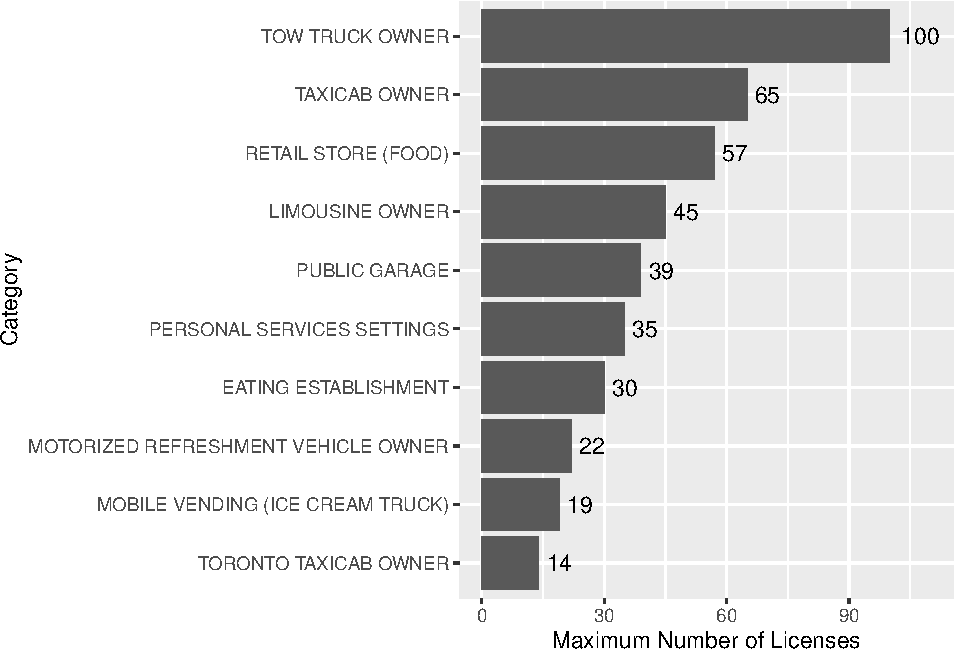
\includegraphics{paper_files/figure-latex/max-1.pdf}
\caption{\label{fig:max}Top 10 Categories with the Highest Maximum Number of Licenses
in a Single Postal Code}
\end{figure}

Figure \ref{fig:max} provides a view of business categories that have the highest concentration within individual postal codes. This can be seen as an indicator of highly localized monopolies or clusters. For example, ``Tow Truck Owner'' tops the chart with a maximum of 100 licenses in a single postal code, followed by ``Taxicab Owner'' with 65 and ``Retail Store (Food)'' with 57.

\textbf{Businesses with Large Fleets}: Businesses like tow truck and taxicab owners tend to cluster heavily in specific postal codes. This could imply the presence of depots or centralized locations for these services.

\textbf{Consumer Essentials}: Retail stores offering food items also show a significant maximum number of licenses in single postal codes, which might indicate areas of high residential density where convenience stores and supermarkets are plentiful.

\textbf{Diverse Services}: The list includes a variety of services from automotive (``Public Garage'') to food and beverages (``Eating Establishment'') and even specific types of vending (``Mobile Vending'').

\newpage

\hypertarget{figure-2-categories-with-the-highest-average-number-of-licenses}{%
\subsection{Figure 2: Categories with the Highest Average Number of Licenses}\label{figure-2-categories-with-the-highest-average-number-of-licenses}}

\begin{figure}
\centering
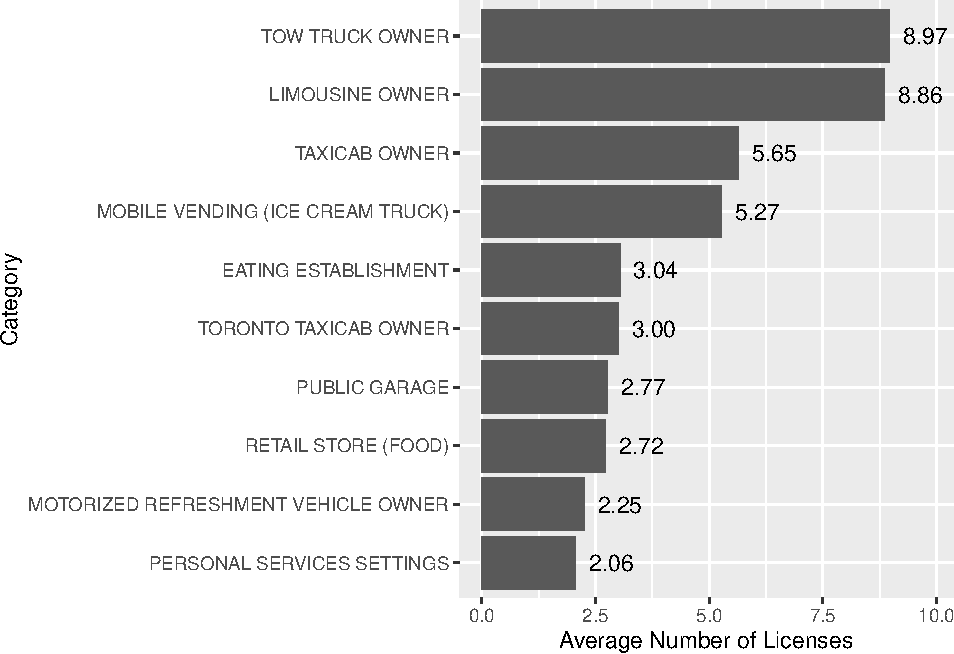
\includegraphics{paper_files/figure-latex/average-1.pdf}
\caption{\label{fig:average}Top 10 Categories with the Highest Average Number of Licenses,
Ignoring Postal Codes with No License of That Particular Category}
\end{figure}

Figure \ref{fig:average} moves from extreme concentration to provide a more balanced view by considering the average number of licenses across all postal codes, excluding those where a particular category is not represented.

\textbf{Consistent Players}: Categories like ``Tow Truck Owner'' and ``Limousine Owner'' appear again, but their numbers are now normalized, giving us a more generalized view of their prevalence.

\textbf{Specialized Services}: Categories such as ``Mobile Vending (Ice Cream Truck)'' make an appearance, showing they have a consistent but specialized presence across multiple areas.

\textbf{Consumer Staples Remain}: The average number of ``Retail Store (Food)'' and ``Eating Establishment'' licenses are still relatively high, further substantiating their widespread existence across the city.

\newpage

\hypertarget{figure-3-categories-with-the-highest-total-number-of-licenses}{%
\subsection{Figure 3: Categories with the Highest Total Number of Licenses}\label{figure-3-categories-with-the-highest-total-number-of-licenses}}

\begin{figure}
\centering
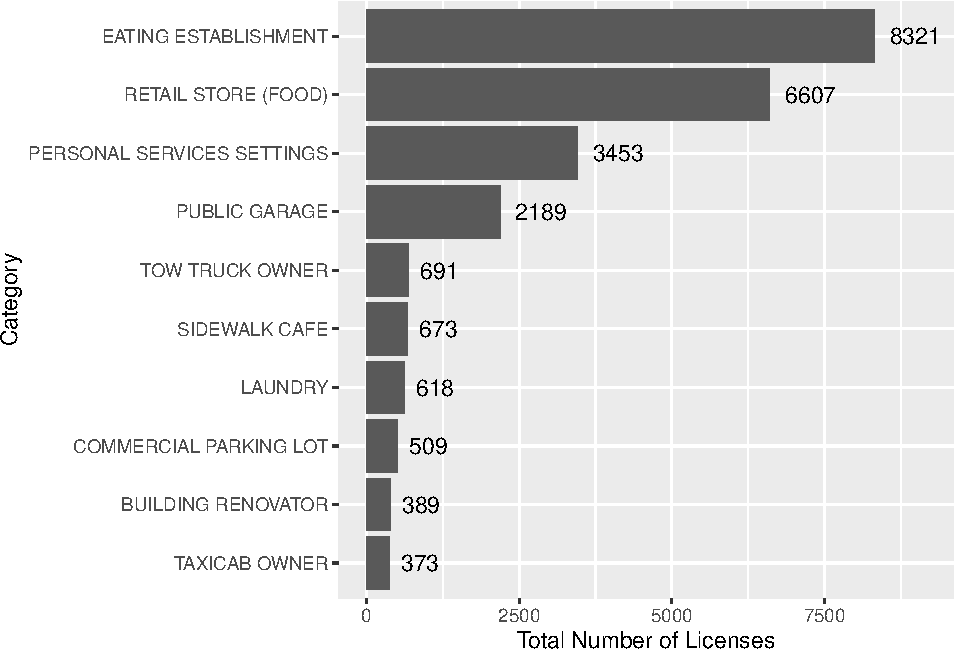
\includegraphics{paper_files/figure-latex/total-1.pdf}
\caption{\label{fig:total}Top 10 Categories with the Highest Total Number of Licenses
among All Postal Codes}
\end{figure}

Figure \ref{fig:total} gives an overall view by showing the total number of licenses across all postal codes for each category.

\textbf{Broad Appeal}: ``Eating Establishment'' and ``Retail Store (Food)'' lead the pack by a significant margin, suggesting that they are omnipresent and cater to a broad consumer base.
\textbf{Essential Services}: Categories like ``Personal Services Settings'' and ``Public Garage'' indicate services that are not only essential but are also widespread.
\textbf{Niche Categories}: Categories like ``Sidewalk Café'' and ``Laundry'' also make the list, showing that specialized businesses too have a notable presence.

\hypertarget{integrated-insights}{%
\subsection{Integrated Insights}\label{integrated-insights}}

\textbf{Overlap and Complementarity}: Businesses like eating establishments and retail food stores appear in all graphs, suggesting that they are not just popular but also well-distributed. The clustering of these business types might suggest a complementary relationship, which could be explored further.

\textbf{Market Saturation}: The high concentration of specific business types like ``Tow Truck Owner'' in some areas may indicate market saturation or potentially high levels of competition.

\hypertarget{correlation-analysis}{%
\section{Correlation Analysis}\label{correlation-analysis}}

The aim of this section is to examine the relationships between different categories of business licenses. Understanding these correlations can provide unique insights into business patterns, zoning considerations, and market dynamics.

\hypertarget{methodology}{%
\subsection{Methodology}\label{methodology}}

The correlation analysis begins with a cleaned dataset of business licenses across various categories and their postal code locations. We then compute a correlation matrix using built-in statistical functions. Unique pairwise combinations of business categories were extracted, and their respective correlation coefficients were calculated. This resulted in a table with three columns: Category A, Category B, and the Correlation Coefficient between them.

\hypertarget{results-and-interpretation}{%
\subsection{Results and Interpretation}\label{results-and-interpretation}}

\hypertarget{top-10-highest-correlation-coefficients}{%
\subsubsection{Top 10 Highest Correlation Coefficients}\label{top-10-highest-correlation-coefficients}}

\begin{table}[H]

\caption{\label{tab:top10}Top 10 Highest Correlation Coefficients}
\centering
\fontsize{10}{12}\selectfont
\begin{tabular}[t]{>{\raggedright\arraybackslash}p{6cm}>{\raggedright\arraybackslash}p{6cm}r}
\toprule
Category A & Category B & Correlation Coefficient\\
\midrule
MOBILE VENDING (ICE CREAM TRUCK) & MOTORIZED REFRESHMENT VEHICLE OWNER & 0.93\\
BUILDING CLEANER & LIMOUSINE OWNER & 0.69\\
TAXICAB OPERATOR & TAXICAB OWNER & 0.65\\
CARNIVAL & CIRCUS & 0.50\\
LIMOUSINE OWNER & LIMOUSINE SERVICE COMPANY & 0.47\\
EATING ESTABLISHMENT & RETAIL STORE (FOOD) & 0.40\\
CURB LANE CAFE & SIDEWALK CAFE & 0.38\\
PERSONAL SERVICES SETTINGS & RETAIL STORE (FOOD) & 0.35\\
EATING ESTABLISHMENT & PERSONAL SERVICES SETTINGS & 0.35\\
EATING ESTABLISHMENT & SIDEWALK CAFE & 0.33\\
\bottomrule
\end{tabular}
\end{table}

Table \ref{tab:top10} shows the business categories with the highest correlation coefficients. Notably, the highest correlation is between ``Mobile Vending (Ice Cream Truck)'' and ``Motorized Refreshment Vehicle Owner'' at 0.93044.

The business categories that appear at the top with high positive correlation coefficients generally belong to related or complementary sectors. For example, ``Mobile Vending'' and ``Motorized Refreshment Vehicle Owner'' both serve food and refreshments in a mobile setting, likely appealing to similar customer bases and benefiting from being in proximity to each other.

The presence of other similar pairings, such as ``Taxicab Operator'' and ``Taxicab Owner'' or ``Limousine Owner'' and ``Limousine Service Company,'' further supports the idea that businesses in the same or complementary sectors tend to establish themselves in similar areas. This could be due to shared operational requirements like zoning laws, similar target demographics, or the advantages of clustering---for example, creating a ``food truck hub'' or ``taxi stand'' that attracts more customer attention than a solitary business could.

\hypertarget{top-10-lowest-correlation-coefficients}{%
\subsubsection{Top 10 Lowest Correlation Coefficients}\label{top-10-lowest-correlation-coefficients}}

\begin{table}[H]

\caption{\label{tab:bottom10}Top 10 Lowest Correlation Coefficients}
\centering
\fontsize{10}{12}\selectfont
\begin{tabular}[t]{llr}
\toprule
Category A & Category B & Correlation Coefficient\\
\midrule
COMMERCIAL PARKING LOT & PUBLIC GARAGE & -0.08\\
PERSONAL SERVICES SETTINGS & PLUMBING CONTRACTOR & -0.08\\
PUBLIC GARAGE & SIDEWALK CAFE & -0.08\\
BUILDING RENOVATOR & PERSONAL SERVICES SETTINGS & -0.08\\
PERSONAL SERVICES SETTINGS & PUBLIC GARAGE & -0.08\\
PLUMBING CONTRACTOR & RETAIL STORE (FOOD) & -0.09\\
COMMERCIAL PARKING LOT & PERSONAL SERVICES SETTINGS & -0.09\\
BUILDING RENOVATOR & RETAIL STORE (FOOD) & -0.10\\
EATING ESTABLISHMENT & PLUMBING CONTRACTOR & -0.12\\
BUILDING RENOVATOR & EATING ESTABLISHMENT & -0.14\\
\bottomrule
\end{tabular}
\end{table}

Table \ref{tab:bottom10} shows the business categories with the lowest correlation coefficients. Most notably, the most negative correlation exists between ``Building Renovator'' and ``Eating Establishment,'' with a coefficient of -0.14225.

On the other end of the spectrum, the business categories with the most negative correlations typically have contrasting needs or target different consumer bases. For instance, ``Building Renovators'' might prefer areas that are under development or renovation and may not be operational during standard business hours, whereas ``Eating Establishments'' would likely want stable, high-traffic areas that are already developed.

However, it's interesting to note that these negative correlations are not as extreme as the positive ones. This suggests that while similar businesses have strong reasons to cluster together, dissimilar businesses don't necessarily avoid each other to the same extent---they may be indifferent to each other's presence rather than antagonistic.

\hypertarget{density-plot-of-correlation-coefficients}{%
\subsubsection{Density Plot of Correlation Coefficients}\label{density-plot-of-correlation-coefficients}}

\begin{figure}
\centering
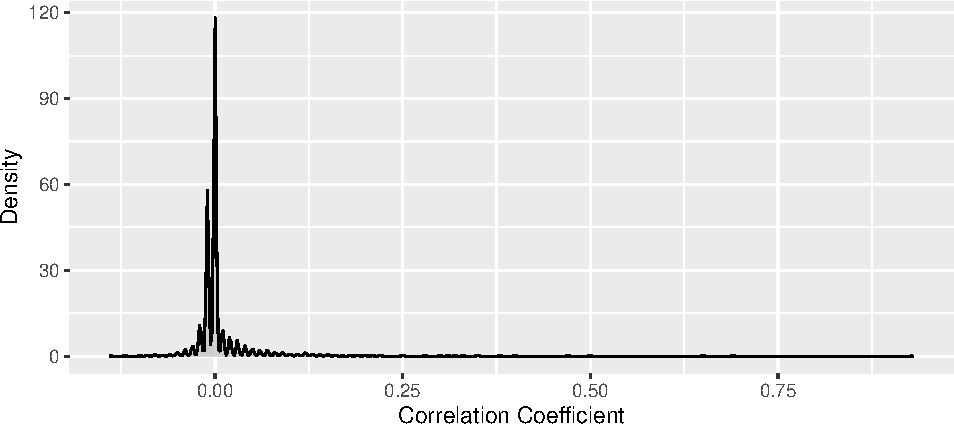
\includegraphics{paper_files/figure-latex/density-1.pdf}
\caption{\label{fig:density}Density Plot of Correlation Coefficients}
\end{figure}

Figure \ref{fig:density} of correlation coefficients reveals a near-normal distribution, skewed slightly towards zero.

The majority of correlation coefficients are near zero, indicating that most business categories don't have a strong inclination to co-locate or avoid each other. However, the extreme positive correlations are much more pronounced than the extreme negative ones.

This pronounced disparity could be attributed to several factors. For one, businesses with high positive correlations might have compelling synergistic reasons to cluster---for instance, shared supply chain requirements, pooled customer bases, or similar regulatory environments. On the other hand, businesses with negative correlations may not have as strong reasons to avoid each other, thus leading to more modest negative coefficients. For example, a high-end boutique and a discount store might not target the same customers but could co-exist in a large shopping area without directly affecting each other's business.

In summary, the businesses at the top of the positive correlation list seem to have concrete, often symbiotic reasons to co-locate, while those at the negative end may simply be avoiding each other due to different target demographics or business needs. However, the lack of extremely negative coefficients suggests that most businesses are more indifferent rather than antagonistic to dissimilar business types when choosing locations.

This enhanced third section aims to provide a more thorough understanding of the correlation coefficients and the underlying reasons for why certain business categories are more likely to be found together or apart.

\hypertarget{statistical-summary}{%
\subsection{Statistical Summary}\label{statistical-summary}}

\begin{table}

\caption{\label{tab:unnamed-chunk-2}Statistical Summary of Correlation Coefficients (Part 1)}
\centering
\begin{tabular}[t]{l|r|r|r|r|r|r|r}
\hline
...1 & vars & n & mean & sd & median & trimmed & mad\\
\hline
X1 & 1 & 2278 & 0.0066533 & 0.0498584 & -0.0026931 & -0.0014627 & 0.0050608\\
\hline
\end{tabular}
\end{table}

\begin{verbatim}
## \vspace{5mm}
\end{verbatim}

\begin{table}

\caption{\label{tab:unnamed-chunk-2}Statistical Summary of Correlation Coefficients (Part 2)}
\centering
\begin{tabular}[t]{l|r|r|r|r|r|r}
\hline
...1 & min & max & range & skew & kurtosis & se\\
\hline
X1 & -0.1422461 & 0.9304364 & 1.072682 & 7.610391 & 95.10072 & 0.0010446\\
\hline
\end{tabular}
\end{table}

The mean correlation coefficient is approximately 0.007, close to zero. This implies that high correlations are generally rare. The 95th percentile has a coefficient of 0.075, further confirming that extreme correlations are unusual.

\hypertarget{discussion}{%
\section{Discussion}\label{discussion}}

One of the primary limitations of this study is the assumption that businesses are operational throughout the entire period of their license validity. While this simplifies the analysis, it may not accurately reflect the complexities of business operations. Another limitation arises from our focus on data from only the year 2022, ignoring the rich historical data that dates back to as early as January 1st, 1948. This temporal limitation precludes us from examining any chronological or causal relationships among businesses over time. Furthermore, our data cleaning process led to the exclusion of potentially insightful variables, such as restrictions on the license or permit, the names under which companies operate, and more granular location data at the street number level. Additionally, using postal codes as geographical units could either dilute or amplify the correlation effect between certain business categories \citep{GRUBESIC2008129}.

Future studies could significantly extend the scope and applicability of this work in several ways. First, a time-series analysis could be conducted to understand how business clusters evolve over time. This could provide insights into whether older businesses tend to attract newer ones within the same or complementary categories. Additionally, future research could incorporate variables that were excluded in this study, such as license restrictions and street-level location data, to provide a more nuanced understanding of business clustering. Moreover, understanding the role of temporal factors, like seasonality or economic cycles, could shed light on the dynamic nature of business clusters. Longitudinal studies that track these variables over time could offer invaluable insights into the external factors that influence the phenomenon of business clustering.

In this study, we delved into the fascinating phenomenon of business clustering within the context of Toronto's licensed businesses. Using data sourced from Toronto's Open Data Portal, specifically from ``Municipal Licensing and Standards - Business Licenses and Permits,'' we analyzed the spatial distribution of various business categories at the postal code level. Our analysis uncovered that out of 3003 unique pairs of business categories, about 1\% exhibited a correlation coefficient higher than 0.194, with the highest being a remarkable 0.930. This suggests that certain types of businesses such as food-related professions tend to co-locate, possibly benefiting from shared resources, customer bases, or other synergistic effects.

However, it's important to acknowledge the limitations of this research, such as the assumption that businesses operate throughout the entire validity period of their licenses, and the exclusion of potentially significant variables.

While these findings offer a starting point, much work remains to be done. Future research could enrich these insights by considering temporal factors, economic cycles, and other external conditions that weren't addressed in this study. Overall, the research serves as a preliminary step in understanding the complex dynamics of business clustering, and we hope it sparks further investigation into this economically and socially significant phenomenon.

\newpage

\appendix

\hypertarget{appendix}{%
\section*{Appendix}\label{appendix}}
\addcontentsline{toc}{section}{Appendix}

You may go to the `outputs\textgreater data\textgreater correlation\_matrix.csv' to review the complete list of combinations and their correlation coefficients.

\newpage

\renewcommand\refname{References}
  \bibliography{references.bib}

\end{document}
